\chapter{Case study: FRP in real-time data flows} % (fold)
\label{sec:uitwerking}

In this chapter a real-time chat application is developed and analyzed. The chat application is implemented twice in different programming styles. The first implementation uses FRP for all application logic and Cycle.js to render to the Document Object Model. The second implementation uses imperative programming for all application logic and JQuery for DOM manipulation.

The backend implementation is the same for both frontend implementations. Real-time communication between server and client is implemented using WebSockets. WebSockets was chosen over HTTP long polling because long polling does not implement a full-duplex communication channel. WebSockets are chosen over WebRTC data channels because of browser support and maturity of the protocol. Furthermore WebRTC is primarily meant for P2P applications and is cumbersome to implement in a client-server architecture \cite{hn}.

The source code of this application is open source and is available on GitHub \cite{chat-code}. The complete frontend application logic from both applications can be found in appendix~\ref{appendix:frp} and \ref{appendix:imp}. Excerpts from the source code are included throughout this chapter to explain implementation details.

\section{User interface}

The application features a very simple user interface (see figure~\ref{figure:chat}). Users can enter their name and a message in the text inputs in the bottom bar. They can then submit the form to send a new message over the WebSocket. The server will then broadcast this message to all clients connected to the WebSocket. 

On the frontend the messages are displayed with an avatar next to them that is automatically generated from the username of the sender. The side the messages are rendered on is dependent on whether the current user is equal to the sender of the message. A user's own messages appear on the right and messages from other people appear on the left.

\begin{figure}[H]
	\centering
	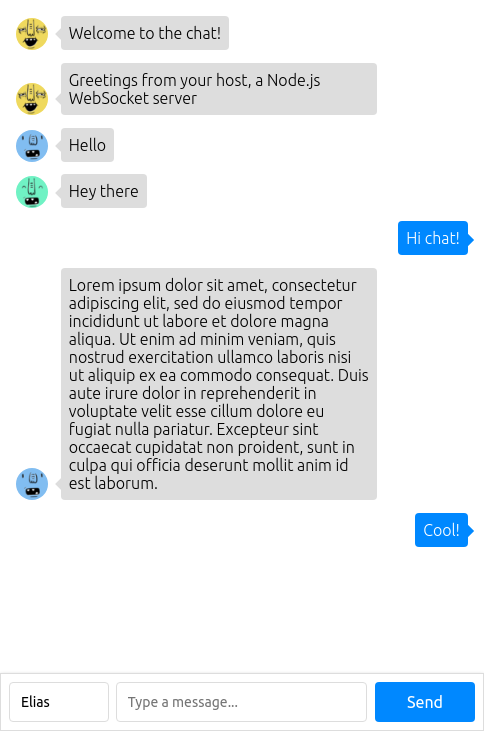
\includegraphics[width=0.6\textwidth]{chat}
	\caption{The chat application interface}
	\label{figure:chat}
\end{figure}

\section{Backend}

\subsection{Implementation}

The backend is implemented in Node.js. It makes use of the Express framework to set up an HTTP server and host the static files from the frontend. The WebSocket implementation that is used is µWebSockets. µWebSockets is a lightweight WebSocket implementation written in C++ with simplicity, performance and scalability as its main objectives \cite{uws}.

µWebSockets was chosen because of its simplicity and performance. This application is meant to be a very minimal implementation of a chat application and as a result it does not need any extra features on top of the WebSocket protocol. Socket.IO or other popular WebSocket libraries would have been overkill for this application as it does not need any of the extra features it provides.

Messages are not persisted on the server because it would add extra dependencies and potential performance bottlenecks. This case study is focused on the comparison of FRP and imperative programming for the web. As a result it was attempted to add as little dependencies as possible to focus on that comparison.

\subsection{Functionality}

The backend sets up the WebSocket using µWebSockets and listens for connections. When a client connects to the WebSocket the server sends out a welcome message. When a client sends a message over the WebSocket the server broadcasts this message to all clients that are currently connected.

\section{Frontend with FRP}
\label{sec:imp-frp}

\subsection{Choice of technologies}

\subsubsection{FRP library}

RxJS is used as the FRP library for this application. This choice is made mainly because of the popularity of the library. ReactiveX is a very mature cross-language FRP library with big companies like Microsoft and Netflix backing it and using it in their own applications \cite{rx}. The JavaScript version of ReactiveX (RxJS) is currently the most popular FRP library for JavaScript by a large margin. The npm installation statistics support this statement \cite{rx-npm}\cite{most-npm}\cite{xs-npm}.

Xstream and Most.js are also considered. Both these FRP libraries feature better performance than RxJS and are only a fraction of the size \cite{rx-npm}\cite{most-npm}\cite{xs-npm}. But ultimately the performance and bundle size of this application is not the priority. Using RxJS has the advantage of more people being familiar with its concepts and operators.

\subsubsection{DOM abstraction}

For a DOM abstraction various frameworks and libraries are considered. Since the objective is to use FRP in the application, frameworks that play nice with FRP have the advantage. Angular is the first framework that comes to mind in this category. Angular has built-in support for observables and even uses RxJS internally for its core APIs. But because of the size and complexity of Angular there is too much overhead for this application. This application is meant to be as minimal as possible and Angular does not fit the bill in that department.

Cycle.js is the next framework to be considered. Cycle.js is a functional and reactive JavaScript framework for predictable code \cite{cycle}. It is written by André Staltz who is also a core contributor of RxJS and the author of xstream \cite{staltz}\cite{xs-npm}. Cycle.js features a very minimal API and allows the programmer to see the application as a pure function. To use Cycle.js the programmer has to only import one function from the framework: \code{run()}. This makes code easy to understand for newcomers since there are no new framework APIs to learn. Cycle.js is also FRP library agnostic and thus allows the programmer to use their library of choice \cite{cycle}.

Because of its minimal API and very functional architecture Cycle.js was chosen as the DOM abstraction for this application. The architecture used in Cycle.js is further explained in  section~\ref{sec:arch}.

\subsection{Architecture}
\label{sec:arch}

Cycle.js lets the developer see the app as a pure function. This \code{main()} function takes source streams as an argument and returns sink streams \cite{cycle}. Figure~\ref{figure:cycle} shows a diagram of how this architecture works in practice.

\begin{figure}[H]
	\centering
	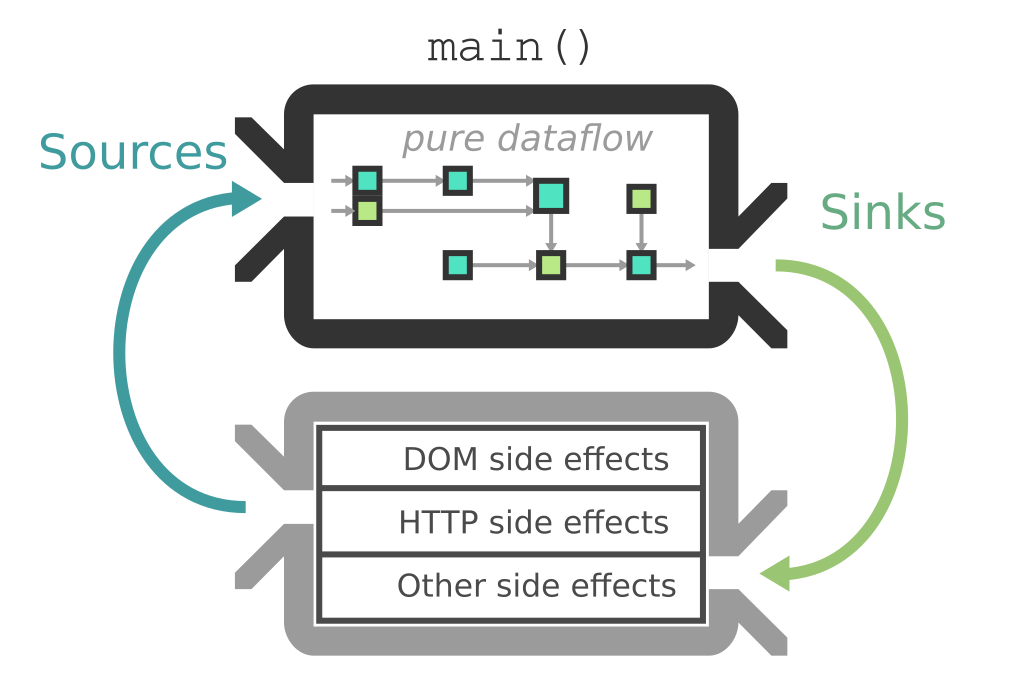
\includegraphics[width=0.8\textwidth]{cycle}
	\caption{Cycle.js application architecture \cite{cycle}}
	\label{figure:cycle}
\end{figure}

The bottom function shown in figure~\ref{figure:cycle} is called a driver. Drivers handle side effects towards various outputs such as the DOM. Drivers take sinks as an argument and return sources for the \code{main()} function to use \cite{cycle-drivers}. Driver functions can be seen as the inverse of the \code{main()} function. Cycle.js provides a few basic drivers for the DOM and for HTTP requests. Cycle.js is very extensible \cite{cycle-drivers} and as a result other drivers written by the community can be found on open source platforms.

\begin{figure}[H]
	\centering
	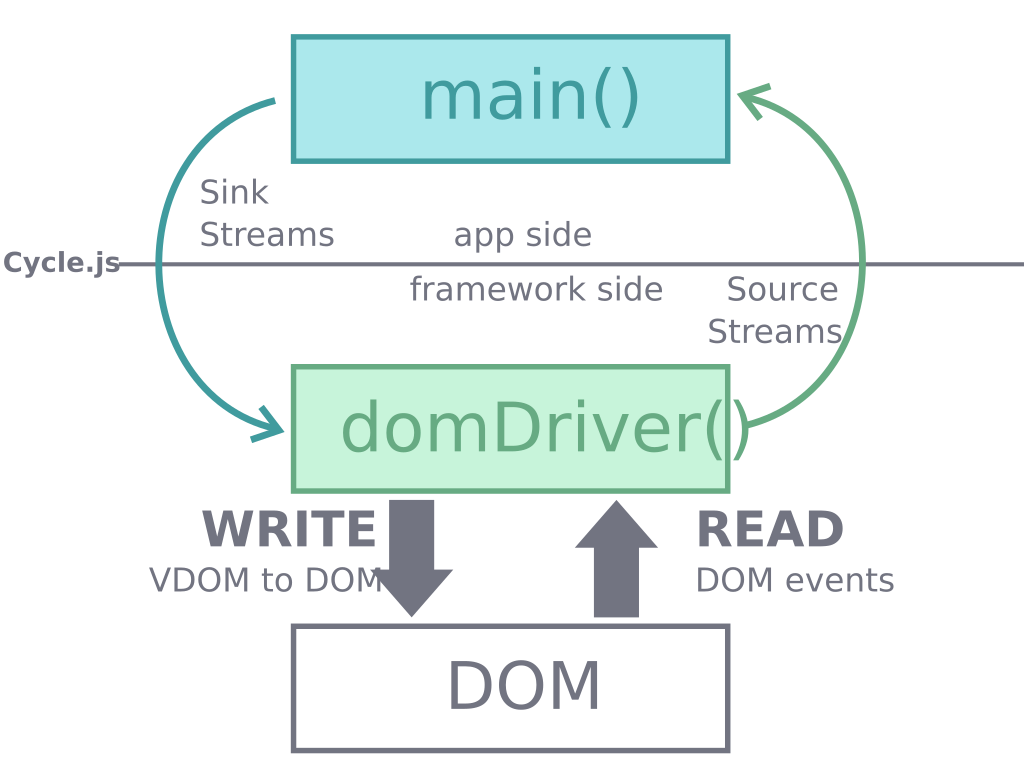
\includegraphics[width=0.7\textwidth]{driver}
	\caption{Cycle.js DOM driver diagram \cite{cycle-drivers}}
	\label{figure:driver}
\end{figure}

The diagram shown in figure~\ref{figure:driver} is an example of a Cycle.js driver. It represents the built-in DOM driver. This driver handles writing DOM changes from the sink stream and provides DOM elements and events in the source stream.

\subsubsection{Custom WebSocket driver}

For this project a custom driver was developed to set the WebSocket up as a source and a sink stream. The driver is available as a package on npm \cite{driver-npm} so that it can be used by other users of Cycle.js. The source code is open source and is available on GitHub \cite{driver-github}.

The driver is a wrapper around the WebSocketSubject object provided by RxJS \cite{ws-subject}. Internally the driver acts as an adapter that forwards the messages from the sink stream to the WebSocketSubject. The driver returns the WebSocketSubject as a whole as the source stream, that way the developer has full control over it in the \code{main()} function. Special attention was given to ensure that the driver is also compatible with other FRP libraries such as xstream and Most.js.

\subsection{Implementation}

When developing an application with the concept of source and sink streams the developer first defines the input streams needed for the application. These input streams can be user input, a real-time database etc.

In the case of this application these input streams are inputs from the user through DOM events and real-time messages from the WebSocket. In the source code the input streams are defined as in listing~\ref{listing:input-streams}. The input streams are derived from the sources given as an argument to the Cycle.js \code{main()} function. In some cases the input streams might even be just a source, without any mutation.

The \code{scan()} operator on the WebSocket source collects all messages received up until this point in an array. The marble diagram in the comment on line 2 shows how this works in practice. \code{\{m\}} represents a single message object.

\begin{lstlisting}[caption=Definition and instantiation of the input streams,label=listing:input-streams]
const messages$ = ws.scan((acc, m) => [...acc, m], []);
// --[{m}]--[{m}, {m}]--[{m}, {m}, {m}]-->
const formSubmit$ = DOM.select('#form').events('submit');
const senderInput$ = DOM.select('#sender').events('input');
const messageInput$ = DOM.select('#message').events('input');
\end{lstlisting}

After the input streams are defined the developer can think about what sinks (output streams) the application will output towards. In the case of web applications one sink that is always used is the DOM. LocalStorage is an example of another output stream that some applications use \cite{local-storage}. In the case of this application the used sinks are the DOM and the WebSocket.

Now that the sources and sinks are known all that is left to do is to combine and manipulate the input streams until they are in the required format for the sinks. Before writing any code it can be useful for the developer to make a dependency graph to see which output streams depend on which input streams. The dependency graph for this chat application is shown in figure~\ref{figure:chat-dep}.

\begin{figure}[H]
	\centering
	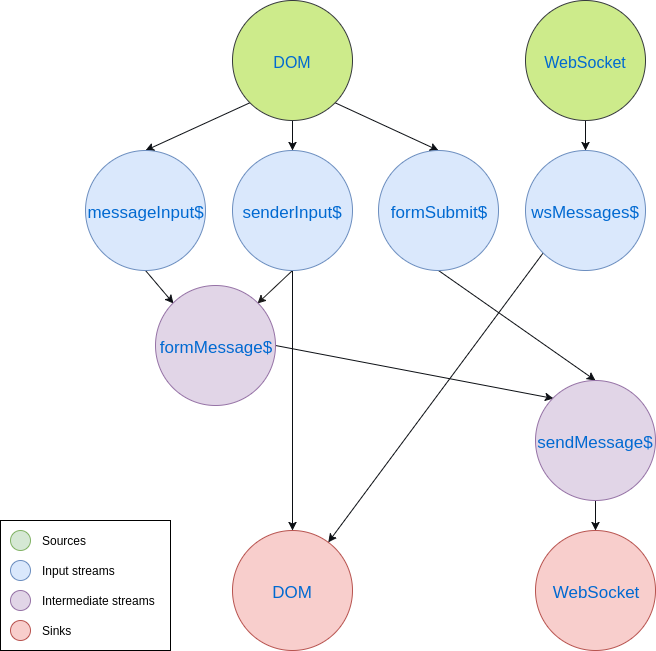
\includegraphics[width=0.7\textwidth]{chatdep}
	\caption{Dependency graph of the chat application}
	\label{figure:chat-dep}
\end{figure}

By using operators to mutate the input streams they are converted to the required format for the output streams. For the sake of readability intermediate streams are used. They are not required but are useful to make reasoning about the application easier. Finally the sinks are handled by the driver functions. The drivers handle all the I/O and side effects caused by the sinks. In the case of the chat application the DOM driver rerenders the DOM with the updated DOM and the WebSocket driver sends newly submitted messages over the WebSocket.

For elegant representation of the DOM in JavaScript, JSX is used. JSX is not a templating language but rather a syntax extension to JavaScript \cite{jsx}. Because of this JSX comes with the full power of JavaScript. JSX was popularized by its use in React \cite{jsx}. In the code we provide the DOM sink as a stream of JSX objects (see listing~\ref{listing:jsx}).

\begin{lstlisting}[caption=Using JSX to define the DOM,label=listing:jsx]
function main({ DOM, ... }) { // sources in function argument
	...
	const vtree$ = Observable
		.combineLatest(wsMessages$.startWith([]), senderInput$.startWith(''))
		.map(([messages, me]) =>
			<div className="wrapper">
				<ul className="chat">
				{ messages && messages.map(m =>
					<li className={`chat__entry${me === m.sender ? ' chat__entry--mine' : ''}`}>
						<span className="chat__entry__message">{m.message}</span>
					</li>
				)}
				</ul>
			</div>
		);
		
	return { DOM: vtree$, ... }; // return sinks
}
\end{lstlisting}

In the code in listing~\ref{listing:jsx} the path towards the DOM sink in the dependency graph shown in figure~\ref{figure:chat-dep} can be recognized. The \code{wsMessages\$} and the \code{senderInput\$} streams are combined to render the current state of the application to the DOM. The \code{startWith()} operators are used to define the initial state.

The JSX in listing~\ref{listing:jsx} in only an excerpt of the complete DOM. Only the logic to render the messages and determine if a message was sent by the current user is included. To render the messages from an array of objects the \code{Array.map()} function is used. This function maps the individual messages to JSX objects. To determine if the current user is the sender of a particular message a ternary is used. The complete source code of this implementation can be found in appendix \ref{appendix:frp}.

\section{Frontend with imperative programming}
\label{sec:imp-imp}

\subsection{Choice of technologies}

When developers create web applications with imperative programming they frequently use libraries such as JQuery as an abstraction over vanilla JavaScript. JQuery makes things like HTML document traversal and manipulation, event handling, animation, and Ajax simpler \cite{jquery}. While there are alternatives to JQuery like Dojo and Ext, JQuery has been and still is the most popular one by far. 

Monolithic abstractions over JavaScript like JQuery have been losing popularity in recent years because of smaller and more modular utility libraries such as lodash. New features and APIs that are added to the JavaScript specification also diminish the need for JQuery. Last but not least more and more developers are migrating to more declarative frameworks and libraries to manipulate the DOM such as React.

For this application JQuery was chosen because it still sees the most usage compared to its competitors. React or Angular are not really options because they are not imperative programming frameworks.

\subsubsection{Templating language}

To render the application to the DOM it was decided to use a templating engine for convenience. Handlebars was chosen as the templating engine for the application. Handlebars provides some utility over Moustache which it is built upon but is still a very minimal templating engine that is much lighter than popular competitors such as Pug \cite{handlebars}. 

\subsection{Architecture}

The application uses a single \code{render()} function that is called whenever the application needs to rerender (see figure~\ref{figure:arch}). The application listens to events from the DOM and from the WebSocket. These events then mutate objects that are stored in globally scoped mutable variables.

\begin{figure}[H]
	\centering
	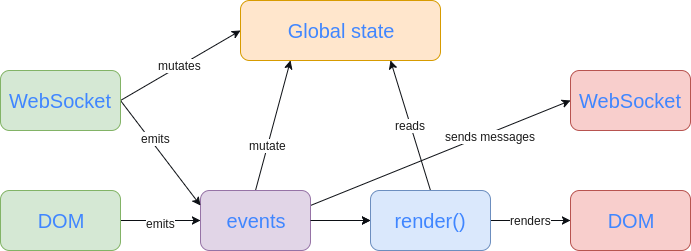
\includegraphics[width=0.9\textwidth]{arch}
	\caption{Diagram of the imperative application architecture}
	\label{figure:arch}
\end{figure}

The event handlers from the \code{onmessage} event on the WebSocket and the \code{oninput} event from the sender input call the \code{render()} function. Whenever the render function gets called it reads variables from the global state and rerenders the application in the DOM. The onsubmit event from the message form causes a new message to be sent over the WebSocket.

\subsection{Implementation}

This implementation uses event handlers to mutate a global state. This global state is instantiated as in listing~\ref{listing:state}.

\begin{lstlisting}[caption=The global variables that make up the application state,label=listing:state]
const template = Handlebars.compile(`
	<div class="wrapper">
		...
	</div>
`);

const messages = [];
let lastMessage = '';
let me = '';
\end{lstlisting}

The \code{messages} variable gets mutated by an event handler on the \code{onmessage} event of the WebSocket. The \code{lastMessage} variable holds the last sent message so that it can be persisted as the input value after render. Lastly the \code{me} variable contains the current sender. This variable is mutated by the event handler on the \code{oninput} event of the text field.

This application architecture is completely different from the FRP implementation. In that implementation the event streams were composed into an unidirectional dataflow (see figure~\ref{figure:chat-dep}). In this implementation event handlers are set up separately. They then all mutate global objects to communicate their data to other parts of the application. 

\subsubsection{Render function}
The \code{render()} function is implemented as shown in listing~\ref{listing:render}.
Internally the render function compiles the Handlebars template with the new data. To have the necessary data the render function first loops over the messages to check which ones are from the current user. Finally it replaces the previous version of the application in the DOM with the newly compiled Handlebars template.

\begin{lstlisting}[caption=Implementation of the render function,label=listing:render]
const render = () => {
	for (let i = 0; i < messages.length; i++) {
		const message = messages[i];
		message.isMine = message.sender === me;
	}
	const data = { messages, me, lastMessage };
	const htmlString = template(data);
	$('#app').html(htmlString);
	$('#sender').focus().val(me);
};
\end{lstlisting}

The last line of listing~\ref{listing:render} covers a corner case where the sender input loses focus while the user is typing because of the rerender. Another corner case that needed to be covered was initial render. Because the \code{render()} function only gets called from events the application would not render until an event occurs. To solve this the \code{render()} function also has to be called on load.  The complete source code of this implementation can be found in appendix \ref{appendix:imp}.

\section{Comparison}

In this chapter the two implementations from section~\ref{sec:imp-frp} and section~\ref{sec:imp-imp} are compared with various metrics. First a static analysis tool is used to analyze the application code. Second the performance of the two applications is compared. Finally some more subjective metrics like readability are discussed.

\subsection{Static analysis}
\label{sec:analysis}

Static analysis of code is the analysis that is performed without executing the program \cite{static}. This type of code analysis is performed on the source code. Static analysis is mostly used to ensure code quality across large code repositories. These tools are typically integrated into the build system and ran automatically for every commit \cite{static}. In the case of this bachelor thesis it is used to compare the two implementations of the chat application.

\subsubsection{Bundle size}

The build system for both frontend implementations is identical. Both use a minimal Webpack setup (see appendix~\ref{appendix:build}). As a result the bundles are generated in the same way. Because of the small size of the application logic the bundle size depends mostly on the imported libraries. To compare and visualize these two bundles the source-map-explorer tool is used. This tool offers an interface to visualize JavaScript bundles and the relative sizes of their contents \cite{sme}.

The JavaScript bundle size of the imperative implementation is approximately 165kB. As can be seen in figure~\ref{figure:imp-smap}, this bundle is split almost evenly between the two dependencies, JQuery and Handlebars.

\begin{figure}[H]
	\centering
	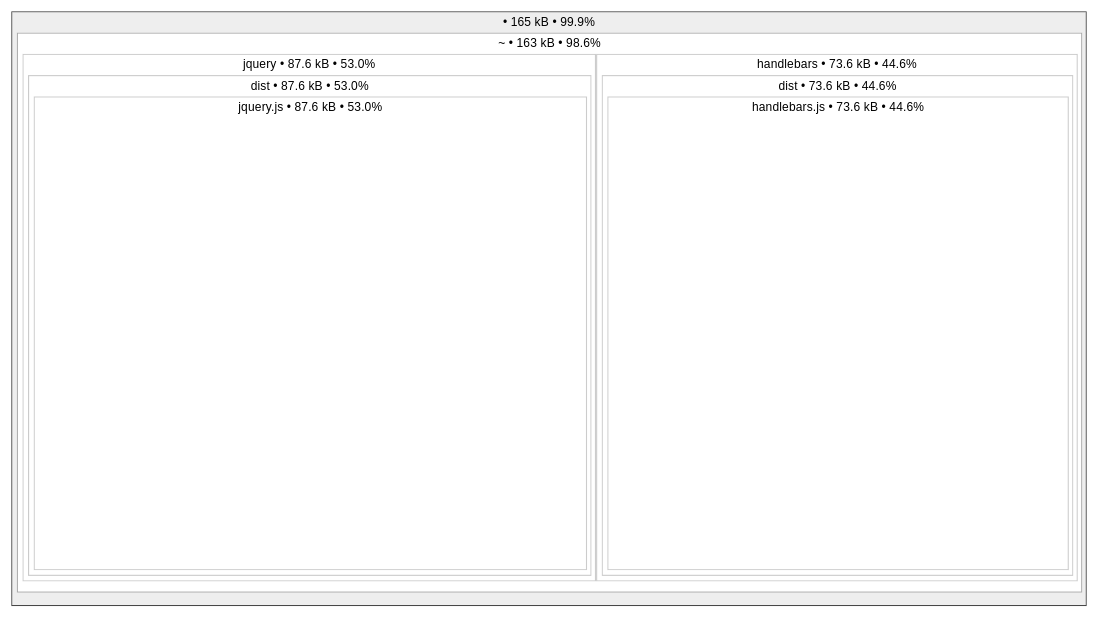
\includegraphics[width=0.8\textwidth]{imp-smap}
	\caption{Visualisation of the JavaScript bundle of the imperative implementation}
	\label{figure:imp-smap}
\end{figure}

The bundle of the FRP implementation is somewhat more complicated. RxJS and Cycle.js are developed in a modular way, this is why importing parts of RxJS can be done with ES2015 module imports as seen in the first 10 lines of appendix~\ref{appendix:frp}. In spite of that RxJS is still the largest dependency in this bundle by far. The total bundle size is 114kB (see figure~\ref{figure:frp-smap}).

Xstream is in this bundle because Cycle.js depends on it \cite{cycle}. If xstream would be used in the application logic this dependency could be reused and more than 43kB could be saved by removing the dependency on RxJS. There are also some polyfills included in this bundle to be compatible with older browsers.

\begin{figure}[H]
	\centering
	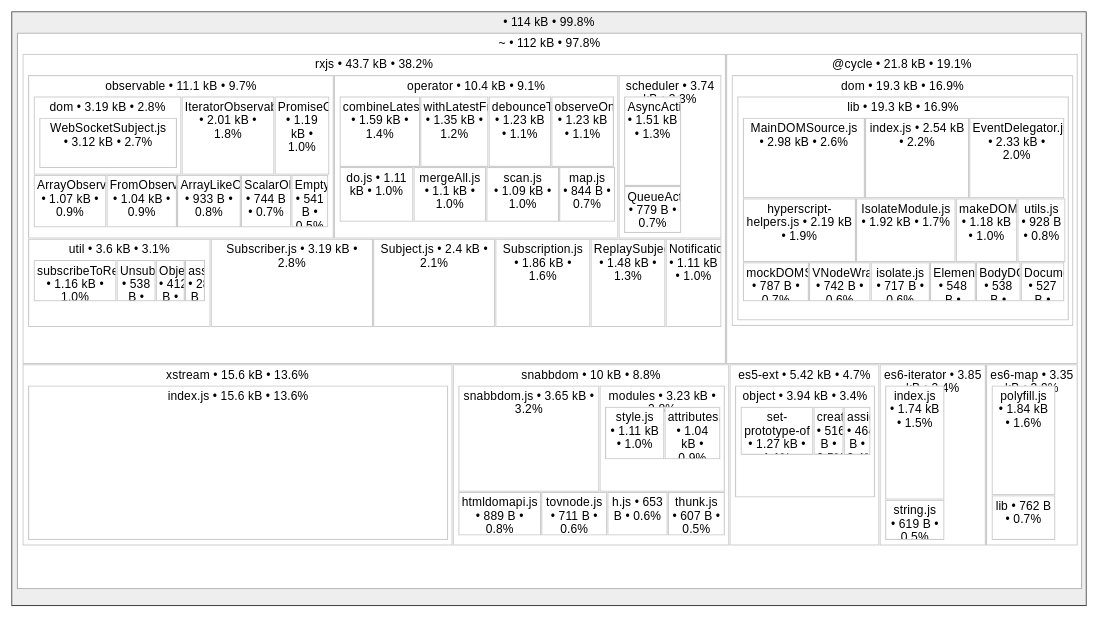
\includegraphics[width=0.8\textwidth]{frp-smap}
	\caption{Visualisation of the JavaScript bundle of the FRP implementation}
	\label{figure:frp-smap}
\end{figure}

\paragraph{Tree shaking}\mbox{}

The build script for this application uses Webpack v1.x which does not support tree shaking. Tree shaking or dead-code elimination relies on the ES2015 module import/export syntax to eliminate unused code \cite{tree-webpack}. By migrating the build script to Webpack v2.x or Rollup, tree shaking can be leveraged to optimize the JavaScript bundle further \cite{tree-webpack}\cite{tree-rollup}.

\subsubsection{Code length}

\paragraph{Simple comparison}\mbox{}

Code length can be evaluated by simply comparing the length of the program in terms of source lines of code (SLOC) and characters. In this calculation empty lines and import statements are excluded. Using this method the FRP implementation is the clear winner. It has only 45 SLOC compared to the imperative implementation's 76 SLOC. The FRP implementation also wins in terms of characters. It counts 1401 characters excluding spaces compared to the imperative implementation's 1797 characters.

\paragraph{Comparison by Halstead measurements}\mbox{}

The comparison in the previous paragraph is valid but not very sophisticated. Character count for example can be heavily influenced by the length of identifiers. But longer identifiers for variables or functions are not necessarily bad, they might make a program more legible. To compare more sophisticated metrics like number of operators and operands Halstead complexity measurements can be used \cite{zuse-halstead}.

To generate these measurements for this application Plato is used. Plato is a tool to report and visualize measurements from static analysis on JavaScript code. These measurements include cyclomatic code complexity and Halstead complexity measures \cite{plato}. The full reports from Plato can be found in appendix~\ref{appendix:plato-frp} and \ref{appendix:plato-imp} in JSON format. The relevant Halstead measurements for code length are displayed in table~\ref{table:hs}.

\begin{table}[H]
	\centering
	\begin{tabular}{|l|c|c|}
		\hline
		\textbf{Metric} & \multicolumn{1}{l|}{\textbf{Imperative implementation}} & \multicolumn{1}{l|}{\textbf{FRP implementation}} \\ \hline
		Number of operands   & 129                                                     & 136                                              \\ \hline
		Distinct operands    & 57                                                      & 72                                               \\ \hline
		Number of operators  & 122                                                     & 116                                              \\ \hline
		Distinct operators   & 20                                                      & 17                                               \\ \hline
		Program length       & 251                                                     & 252                                              \\ \hline
		Physical SLOC        & 87                                                      & 58                                               \\ \hline
		Logical SLOC         & 39                                                      & 15                                               \\ \hline
		Volume               & 1573                                                    & 1631                                             \\ \hline
		Vocabulary           & 77                                                      & 89                                               \\ \hline
	\end{tabular}
	\caption{Halstead measurements for both implementations (Lower is better)}
	\label{table:hs}
\end{table}

The number of operands and operators is almost equal for both implementations. The FRP implementation has slightly more operands and slightly less operators compared to the imperative implementation. As a result the Halstead program length (sum of total operands and operators) is as good as equal for both implementations.

Logical SLOC is an interesting measurement. It counts the number of imperative statements and not the number of lines like physical SLOC \cite{complexity}. Unsurprisingly the FRP implementation has less imperative statements than the imperative implementation. In fact the Logical SLOC of the FRP implementation is less than half of the logical SLOC of the imperative implementation.

The FRP implementation has more vocabulary and a higher volume than the imperative implementation. The Halstead vocabulary is simply the sum of the number of distinct operators and operands \cite{ibm-halstead}. This is higher for the FRP implementation because of the high number of distinct operators it introduces. This might contribute to the steep learning curve for learning FRP. The Halstead volume is calculated from the program length and the vocabulary \cite{ibm-halstead}. This measurement being higher for the FRP implementation is simply a result of the volume being higher.

\subsubsection{Cyclomatic complexity}

Cyclomatic complexity is a source code complexity metric to measure the number of independent paths execution can take through a program \cite{cyclo}. Cyclomatic complexity is calculated by constructing the control flow graph of a program. For a single function the cyclomatic complexity is then calculated by the following formula: $M = E - N + 2$ \cite{cyclo}. In that formula M stands for the cyclomatic complexity, E for the number of edges of the control flow graph and N for the number of nodes in the graph. Figure~\ref{figure:cfg} shows the control flow graph of a simple example program shown in listing~\ref{listing:cfg}. 

\begin{figure}[H]
	\centering
	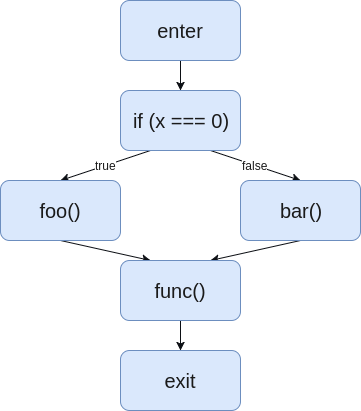
\includegraphics[width=0.4\textwidth]{cfg}
	\caption{Control flow graph of a simple program (see listing~\ref{listing:cfg})}
	\label{figure:cfg}
\end{figure}

Using the aforementioned formula on this function results in a cyclomatic complexity of 2 (6 - 6 + 2). This makes sense because there are only two possible paths through this code. One where the if statement is true and one where it is false.

\begin{lstlisting}[caption=Example code to illustrate the calculation of cyclomatic complexity,label=listing:cfg]
function run(x) {
	if (x === 0) {
		foo();
	} else {
		bar();
	}
	func();
}
\end{lstlisting}

The cyclomatic complexities of the two implementations are both relatively low. The FRP implementation has a cyclomatic complexity of 3 and a density of 20. The density of cyclomatic complexity is calculated by comparing it with the SLOC \cite{cyclo}. The imperative implementation has a higher complexity (5) but a lower density (12.8).

\paragraph{Plato metrics}\mbox{}

The Plato tool provides a number of different metrics to indicate code quality. Most of them are Halstead complexity measurements. Table~\ref{table:plato} shows a selection of the most relevant measurements for both implementations.

\begin{table}[H]
	\centering
	\begin{tabular}{|l|c|c|}
		\hline
		\textbf{Metric}  & \multicolumn{1}{l|}{\textbf{Imperative implementation}} & \multicolumn{1}{l|}{\textbf{FRP implementation}} \\ \hline
		Difficulty (Halstead) & 23                                                      & 16                                               \\ \hline
		Effort (Halstead) & 35599                                                      & 26201                                               \\ \hline
		Time (Halstead)       & 1977                                                    & 1455                                             \\ \hline
		Maintainability       & 70                                                      & 83                                               \\ \hline
	\end{tabular}
	\caption{Plato measurements for both implementations}
	\label{table:plato}
\end{table}

The Halstead difficulty measures how difficult it is to write a program. This measurement is calculated from the number of operators and operands \cite{ibm-halstead}. According to this measurement the FRP implementation is significantly less difficult to program.

The Halstead effort is the product of the Halstead difficulty and volume. The Halstead time is a weighted version of the effort \cite{zuse-halstead}. It is meant as an approximation of the time it would take to write a program in seconds. Since the difficulty and the volume of the imperative implementation are both higher than those of the FRP implementation the effort and time measurements are also higher. In fact this measurement indicates that the imperative implementation requires 26\% more effort to program. 

Maintainability is a logarithmic scale from negative infinity to 171 introduced by Paul Oman and Jack Hagemeister in 1991 \cite{zuse-halstead}. It is calculated from the logical SLOC, the cyclomatic complexity and the Halstead effort \cite{zuse-halstead}. All of these measurements are worse for the imperative implementation. As a result it scores significantly worse than the FRP implementation for maintainability.

\subsection{Performance}

To compare the performance of these two implementations two usage scenarios are evaluated. To measure performance Chrome Devtools is used.

\subsubsection{Initial load}

The imperative implementation loads significantly faster than the FRP implementation (see figure~\ref{figure:load-frp} and \ref{figure:load-imp}). The imperative application loads in 182ms whereas the FRP application loads in 209ms. These times are measured from the time of the initial HTTP request until the DOMContentLoaded event. This result is surprising considering the bundle of the imperative application is bigger than the FRP bundle (see section~\ref{sec:analysis}). 

\begin{figure}[H]
	\centering
	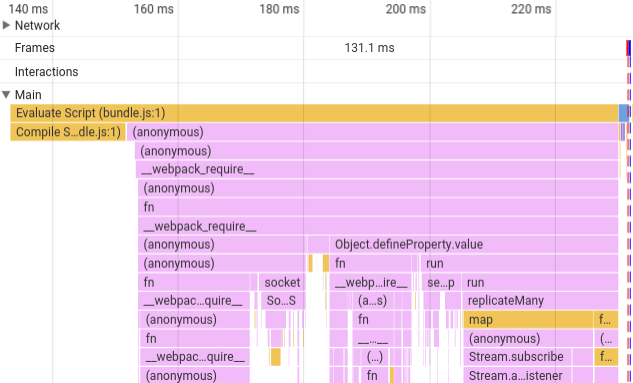
\includegraphics[width=0.7\textwidth]{load-frp}
	\caption{Devtools timeline of initial load in the FRP application}
	\label{figure:load-frp}
\end{figure}

This difference can be explained by the internal work Cycle.js is doing on startup. Cycle.js needs to initialize the source and sink streams for the application as well as its DOM driver. The Cycle.js DOM driver uses a virtual DOM implementation to optimize the changes it does to the DOM. This means that it has to load a representation of the DOM into memory on initial load. After all that work is completed it can run the \code{main()} function to do the initial render of the application.

\begin{figure}[H]
	\centering
	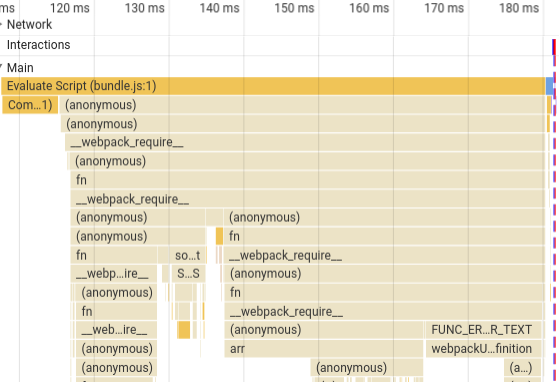
\includegraphics[width=0.7\textwidth]{load-imp}
	\caption{Devtools timeline of initial load in the imperative application}
	\label{figure:load-imp}
\end{figure}

The work done in the imperative application is considerably less complex. The only thing the application does on initial load is instantiating some variables to hold the global state and then calling the \code{render()} function. The render function then runs the templating engine with the data from the initial global state and injects it into the DOM. This application keeps no virtual representation of the DOM in memory.

Memory consumption is almost equal for both implementations (see figure~\ref{figure:mem-frp} and \ref{figure:mem-imp}). Interestingly the imperative application mounts 114 more DOM nodes than the FRP implementation even though HTML markup is identical for both applications.

\begin{figure}[H]
	\centering
	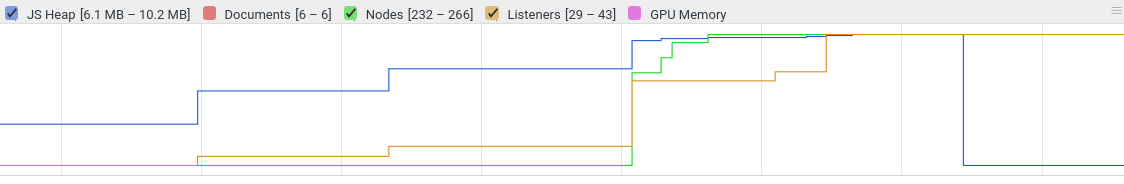
\includegraphics[width=\textwidth]{mem-frp}
	\caption{Memory allocation when loading the FRP application}
	\label{figure:mem-frp}
\end{figure}

\begin{figure}[H]
	\centering
	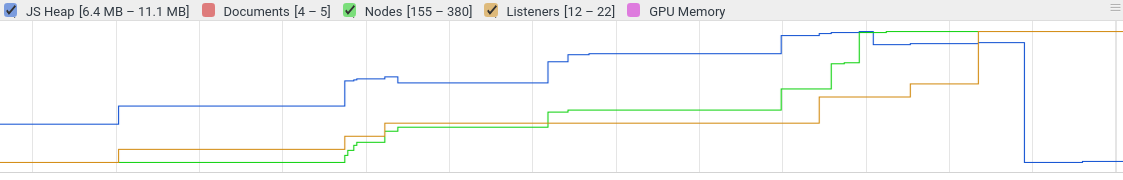
\includegraphics[width=\textwidth]{mem-imp}
	\caption{Memory allocation when loading the imperative application}
	\label{figure:mem-imp}
\end{figure}

The difference can be explained by the optimization of the Cycle.js DOM driver. This driver calculates the difference of the current DOM state and the new state using its virtual DOM. As a result it only replaces the nodes in the DOM that have changed. The imperative implementation does not have these optimizations and just replaces all the DOM nodes in the application. The reason why the application is rerendered a few times on load is because the server sends welcome messages over the WebSocket.

\subsubsection{Adding a message}

In this scenario the applications need to debounce the submit event of the message form and then send the message over the WebSocket. When the server broadcasts this message to them they need to render it in the DOM. In figure~\ref{figure:add-frp} and \ref{figure:add-imp} the Chrome Devtools timeline for both applications is shown.

\begin{figure}[H]
	\centering
	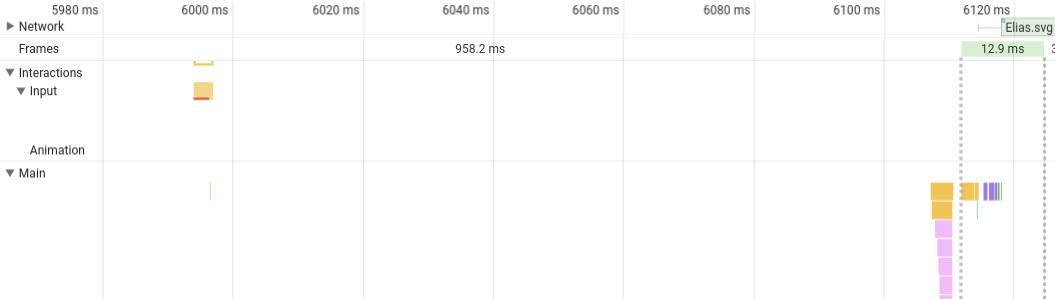
\includegraphics[width=0.9\textwidth]{add-frp}
	\caption{Devtools timeline when adding a message in the FRP application}
	\label{figure:add-frp}
\end{figure}

The first yellow section that is visible in the input row on both timelines is the submit event from the form. After the event a delay follows because of the debounce function. The sending of the message over the WebSocket is very fast in both implementations but the imperative implementation is faster. The imperative implementation does it in 1.8ms and the FRP version in 3.5ms. That is a result of the imperative implementation using the native WebSocket API directly. The FRP implementation uses an abstraction layer from RxJS on top of that API \cite{ws-subject}.

\begin{figure}[H]
	\centering
	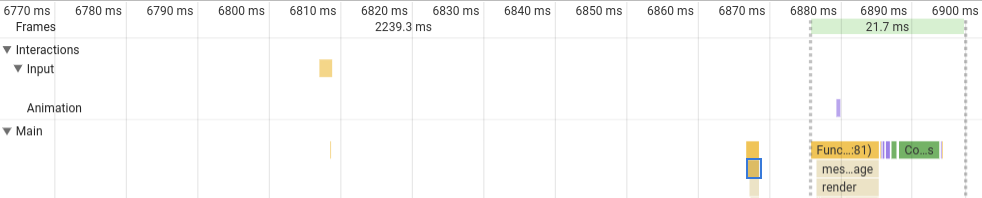
\includegraphics[width=0.9\textwidth]{add-imp}
	\caption{Devtools timeline when adding a message in the imperative application}
	\label{figure:add-imp}
\end{figure}

Receiving and rendering the message is considerably slower in the imperative application. It takes 21.7ms to receive the message and render it to the DOM. 21.7ms of processing time means that the browser momentarily dipped below 60fps. This could cause stuttering animation in the application. The FRP application only takes 12.9ms and stays comfortably above 60fps.

This difference can be explained by the more efficient DOM rendering done internally by Cycle.js. Because of its virtual DOM it only replaces the DOM nodes that need to be replaced. A lot of these performance measurements depend heavily on framework specific implementations. In section~\ref{sec:inf} this is discussed further and a third implementation in vanilla JavaScript without any dependencies is compared.

\subsection{Readability}

Readability of a program is arguably more important than performance or efficiency. An argument for this is that programmers spend a lot of time reading code, arguably more time than they spend writing it \cite{read}. Developers read code when debugging, doing peer reviews and learning new libraries. Because applications are almost always written by multiple developers it is important that code is readable and understandable. The consensus in the industry is that optimizing for readability is more beneficial than optimizing for performance \cite{read}.

In general there are two factors that make code less readable. The code can be hard to understand or it can be hard to follow. Code can be hard to understand if it tries to be too clever or does undocumented low-level optimizations. Code is hard to follow if there is no clear structure or architecture. It can also be hard to follow if the code execution is disconnected. In this case disconnected means that it is not possible to step through the code and follow the order of execution \cite{read}.

The FRP implementation follows an unidirectional dataflow. This architecture allows the developer to see the program as a pipeline. Data flows through each pipe and is mutated and combined with data from different pipes. This makes an application easy to reason about and easy to visualize with a marble diagram or a dependency graph. The catch is that being able to understand this code requires knowledge of the FRP paradigm and of the API of an FRP library.

The imperative implementation mutates a global state through multiple event handlers. This makes this implementation harder to follow. Different event handlers might be mutating the same object and it is hard to deal with this concurrency. When trying to follow this code the reader needs to constantly jump between global variables and the functions they are mutated from. Composing these events into a single flow is not possible without the FRP paradigm. Especially when the application deals with real-time data such as data from WebSockets it becomes cumbersome to manage all these events.

\subsection{Influence of dependencies on results}
\label{sec:inf}

Choice of frameworks and libraries has a big influence on the comparison done in this chapter. Especially the performance section depends almost entirely on the implementation of the library. Because of this a third implementation is developed. This implementation also uses imperative programming but uses no dependencies. It would be useful to also have an FRP implementation without any dependency to compare with but unfortunately there is no support for an observable data structure built in to JavaScript (yet \cite{tc39}). The complete implementation in vanilla JavaScript is available in appendix~\ref{appendix:vanilla}. The most important metrics from static and performance analysis are shown in table~\ref{table:vanilla}.

\begin{table}[H]
	\centering
	\begin{tabular}{|l|c|c|c|}
		\hline
		\multicolumn{1}{|c|}{\textbf{Metric}} & \textbf{\begin{tabular}[c]{@{}c@{}}Imperative\\ implementation\\ (vanilla JS)\end{tabular}} & \textbf{\begin{tabular}[c]{@{}c@{}}Imperative\\ implementation\\ (JQuery)\end{tabular}} & \textbf{\begin{tabular}[c]{@{}c@{}}FRP\\ implementation\end{tabular}} \\ \hline
		Bundle size & 1.8kB & 165kB & 114kB \\ \hline
		Maintainability & 69 & 70 & 83 \\ \hline
		Program length (Halstead) & 469 & 251 & 252 \\ \hline
		Time (Halstead) & 5860 & 1977 & 1455 \\ \hline
		Logical SLOC & 78 & 39 & 15 \\ \hline
		Cyclomatic complexity & 9 & 5 & 3 \\ \hline
		Initial load duration & 147ms & 182ms & 209ms \\ \hline
		Send message duration & 0.4ms & 1.8ms & 3.5ms \\ \hline
		Render new message duration & 9.5ms & 21.7ms & 12.9ms \\ \hline
	\end{tabular}
	\caption{Summary of metrics from static and performance analysis}
	\label{table:vanilla}
\end{table}

The vanilla JavaScipt implementation bundle is only a fraction of the size of the bundle of the other two implementations because it has no dependencies. On all performance metrics it is faster than the other two. This makes sense because it is directly using the native browsers APIs instead of abstractions.

All these size and performance winnings come at the cost of extra code complexity. The cyclomatic complexity is almost twice as high as the imperative implementation with JQuery. All Halstead metrics are also considerably worse for this implementation. The Halstead time is almost 3 times as high as the JQuery implementation and more than 4 times as high as the FRP implementation. This indicates that this version of the application would take 4 times longer to write than the FRP implementation. This increased overall complexity and length also has a negative impact on readability.